\chapter{Espacio local del objeto}
\section{Diferencias entre espacio local y espacio global}
Las posiciones 3D y las transformaciones existen dentro de un sistema de coordenadas llamados \textit{espacios}.

El \textbf{espacio global} es el sistema de coordenadas para la escena entera. Su origen está en el centro de la escena.

El \textbf{espacio local del objeto} es el sistema de coordenadas desde el punto de vista del objeto. El origen del espacio local del objeto está en el centro del mismo, y sus ejes son rotados con el objeto. Tanto en OpenGL como en la librería gráfica propia el concepto de \textit{objeto} es simplemente una lista ordenada de vértices. Esto es llamado \textit{Primitive}. El proceso de creación de estas listas ordenadas de vértices se llama \textit{Vertex Specification}. Los vértices se relacionan de una forma u otra dependiendo del tipo de \textit{primitive} que componen. 

\newpage

\newgeometry{top=20mm, bottom=40mm}

\section{Tipos de primitivos}

\subsection{Primitivos de puntos}
\begin{itemize}
\item{GL\_POINTS: se interpreta cada vértice individual como un punto.}

\end{itemize}

\begin{figure} [h]
  \centering
  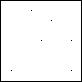
\includegraphics[width=0.3\textwidth]{gl_points}
  \caption{GL\_POINTS}
\end{figure}

\subsection{Primitivos de líneas}
\begin{itemize}
\item{GL\_LINES: Los vértices 0 y 1 se consideran una línea. Los vértices 2 y 3 se consideran una línea, y así progresivamente. Si el usuario especifica un número impar de vértices, el vértice extra es ignorado.}
\item{GL\_LINE\_STRIP: Los vértices adyacentes se consideran líneas. Entonces, si se pasan \textit{n} vértices, se producen \textit{n}-1 líneas. Si el usuario sólo pasa una línea se ignora el comando de dibujo.}
\item{GL\_LINE\_LOOP: Como el anterior excepto que el primer y último vértice también són usados como línea. Entonces, se producen \textit{n} líneas para \textit{n} vértices de entrada.}
\end{itemize}


\begin{figure} [h]
  \centering
  \captionsetup[subfigure]{justification=centering}
  \begin{subfigure}  {0.3\textwidth}
    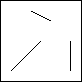
\includegraphics[width=\textwidth]{gl_lines}
    \caption{GL\_LINES}
  \end{subfigure}
  \begin{subfigure} {0.3\textwidth}
    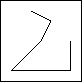
\includegraphics[width=\textwidth]{gl_line_strip}
    \caption{GL\_LINE\_STRIP}
  \end{subfigure}
  \begin{subfigure} {0.3\textwidth}
    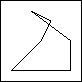
\includegraphics[width=\textwidth]{gl_line_loop}
    \caption{GL\_LINE\_LOOP}
  \end{subfigure}
  \caption{Primitivos de líneas}
\end{figure}

\restoregeometry


\newpage

\newgeometry{top=10mm, bottom=20mm}


\subsection{Primitivos triangulares}
Un triangulo es un primitivo formado por 3 vértices. Es la forma bidimensional con el menor número de vértices, así que los renderizadores normalmente están diseñados para rendierizar con ellos.
\begin{itemize}
\item{GL\_TRIANGLES: Los vértices 0, 1 y 2 forman un triángulo, Los vértices 3, 4 y 5 forman un triángulo, y así progresivamente.}
\item{GL\_TRIANGLE\_STRIP: Cada grupo de 3 vértices adyacentes forma un triángulo. Una lista de \textit{n} vértices forma \textit{n}-2 triángulos.}
\item{GL\_TRIANGLE\_FAN: El primer vértice siempre se mantiene fijo. De ahí en adelante, por cada grupo de dos vértices adyacentes se hará un triángulo con el primero. Una lista de \textit{n} vértices generará \textit{n}-2 triángulos.}
\end{itemize}

\begin{figure} [ht]
  \centering
  \captionsetup[subfigure]{justification=centering}
  \begin{subfigure} {0.3\textwidth}
    
\includegraphics[width=\textwidth]{gl_triangles}
    \caption{GL\_TRIANGLES}
  \end{subfigure}
  \begin{subfigure} {0.3\textwidth}
    
\includegraphics[width=\textwidth]{gl_triangle_strip}
    \caption{GL\_TRIANGLE\_STRIP}
  \end{subfigure}
  \begin{subfigure} {0.3\textwidth}
    
\includegraphics[width=\textwidth]{gl_triangle_fan}
    \caption{GL\_TRIANGLE\_FAN}
  \end{subfigure}
  \caption{Primitivos triangulares}
\end{figure}

\subsection{Primitivos \textit{quad}}
Un \textit{quad} es un primitivo cuadrilateral de cuatro vértices. Frecuentemente se tratan como un par de triangulos.
\begin{itemize}
\item{GL\_QUADS: Vértices 0-3 forman un quad, vértices 4-7 forman otro, y así progresivamente. El número de vértices en la lista debe de ser divisible por 4 para funcionar.}
\item{GL\_QUAD\_STRIP: De forma similar a GL\_TRIANGLE\_STRIP, un \textit{quad strip} utiliza los bordes adyacentes para formar el siguiente quad. En el caso de los quads, el tercer y cuarto vértice de un quad se utilizan para el siguiente \textit{quad}. De esta forma, los vértices 0-3 son un quad, 2-6 son otro quad y así progresivamente. Una lista de \textit{n} vértices generará \textit{n}-2 / 2 quads.}
\end{itemize}

\begin{figure} [h]
  \centering
  \captionsetup[subfigure]{justification=centering}
  \begin{subfigure}{0.3\textwidth} 
    
\includegraphics[width=\textwidth]{gl_quads} 
    \caption{GL\_QUADS}
  \end{subfigure}
  \begin{subfigure}{0.3\textwidth}
    
\includegraphics[width=\textwidth]{gl_quad_strip} 
    \caption{GL\_QUAD\_STRIP}
  \end{subfigure}
  \caption{Primitivos \textit{quad}}
\end{figure}

\restoregeometry

\section{Especificación de vértices usando la librería gráfica}
Es importante destacar que desde que se inicia la creación de un \textit{primitive} hasta que se termina \textbf{no} se puede utilizar una función de transformación.

\subsection{Inicio del \textit{primitve}}
Para iniciar la especificación de vértices hace falta llamar a la siguiente función
\begin{lstlisting}[language=C]
  glBegin(GLEnum mode)
\end{lstlisting}
Y como único argumento introducimos el tipo de primitivo (ver sección anterior).

\subsection{Pasar coordenadas de los vértices}
Existen diversas funciones para crear vertices, dependiendo de si quieren utilizar numeros flotantes o enteros, y si se quieren utilizar tres dimensiones o solo dos. Esas funciones son las siguientes.
\begin{lstlisting}[language=C]
  glVertex2f(GLfloat x, GLfloat y);
  glVertex2i(GLint x, GLint y);
  glVertex3f(GLfloat x, GLfloat y, GLfloat z);
  glVertex3i(GLint x, GLint y, GLint z);
\end{lstlisting}

\subsection{Pasar color de los vértices}
Cada vértice tiene un color con unos valores RGBA concretos, para asignarlos se usa una de las siguientes funciones.
\begin{lstlisting}[language=C]
  glColor3f(GLfloat red, GLfloat green, GLfloat blue);
  glColor3i(GLint red, GLint green, GLint blue);
  glColor4f(GLfloat red, GLfloat green, GLfloat blue, GLfloat alpha);
  glColor4i(GLint red, GLint green, GLint blue, GLfloat alpha);
\end{lstlisting}
De forma similar a pasar coordenadas a los vértices, existen diferentes funciones dependiendo de si se quiere pasar el valor \textit{alpha} o no, y dependiendo de el tipo de número.

Cabe destacar que con llamar a esta función una vez se aplica a todos los vértices especificados posteriormente (incluso si forman parte de otro primitivo) hasta que se vuelve a llamar la función con otro color.
\subsection{Finalizacion del \textit{primitive}}
Una vez que se han terminado de introducir los vertices, hace falta llamar a la siguiente funcion sin ningun argumento.
\begin{lstlisting}[language=C]
  glEnd();
\end{lstlisting}
